\documentclass{article}

\usepackage[affil-it]{authblk}
\usepackage{lineno}
\usepackage{soul}
\usepackage{color}
\usepackage[utf8]{inputenc}
\usepackage[T1]{fontenc}
\usepackage[square,numbers,sort&compress]{natbib}

\usepackage{amsthm}
\usepackage{amssymb}
\usepackage{mathtools}
\usepackage{mathabx}
\usepackage{bm}

\newcommand{\pos}{\mathbf{x}}
\newcommand{\pvel}{\boldsymbol{\xi}}
\newcommand{\mvel}{\mathbf{u}}
\newcommand{\cop}{\boldsymbol{\Omega}}
\newcommand{\grad}{\boldsymbol{\nabla}}
\newcommand{\mmom}{\mathbf{j}}
\newcommand{\transM}{\mathbf{M}}

\title{Accuracy, Stability, and Efficiency of Lattice Boltzmann Models in Simulating Non-Newtonian Flow}
%\title{A Comparison of Lattice Boltzmann Method Collision Operators for Accuracy, Stability and Efficiency in Simulating Non-Newtonian Flows}

\author{{Matthew Grasinger}
\thanks{Email: \textit{grasingerm@pitt.edu}}}

\author{{Scott Overacker}
\thanks{Email: \textit{sdo10@pitt.edu}}}

\author{John Brigham
\thanks{Email: \textit{brigham@pitt.edu}}}
\affil{Civil and Environmental Engineering Department, University of Pittsburgh}

\begin{document}

\pagenumbering{gobble}
\maketitle
\newpage
\tableofcontents
\newpage
\pagenumbering{arabic}

\linenumbers

Note: anything in {\color{red}red} is just random garbage notes.
You can ignore it for the most part.

\section*{Abstract}

The Lattice Boltzmann method (LBM) is a computational method that can be used for simulating fluid flow.
It is well-suited for complex flows such as non-Newtonian, free surface, and multiphase multicomponent flows.
Non-Newtonian flows are the primary focus of this paper, as many practical engineering problems such as the flow of cement slurries and concretes, the filling of molds by molten metals and plastics, blood flows, etc., are best modeled as non-Newtonian fluids.
LBM is a statistical mechanical approach for simulating fluid flow.
Each time step consists of streaming particle distributions to neighboring nodes, and collisions of particle distributions at each node through a collision operator.
The collision operator is of interest because it has a lot of control over the physics that are simulated, e.g. constitutive laws, interfacial dynamics, etc., and it has implications on numerical stability and computational efficiency.
In this paper, various collision operators and methods for stability enhancement will be examined for their suitability for simulating non-Newtonian flows in terms of accuracy, numerical stability and computational efficiency.
The structure of the paper will be as follows: blah, blah, blah.

\section{Introduction} %MG: this intro will potentially be long. Should it be broken up into subsections (as it is now)?

\subsection{Applications of Non-Newtonian Flow}

The dynamic viscosity of a fluid is a measure of its resistance to shear deformation.
For many fluids, at a constant temperature, the dynamic viscosity can be considered as constant.
These fluids are known as Newtonian fluids.
Non-Newtonian fluids have an apparent dynamic viscosity, or apparent resistance to shear stress, that is variable--even at a constant temperature--and is often a function of strain-rate.
There are a number of fluids in science and engineering applications that can be classified as non-Newtonian; pastes, slurries, molten plastics, polymer solutions, dyes, varnishes, suspensions, and some biomedical liquids such as blood all behave in a non-Newtonian manner \cite{bohme1987non}.
Of all of the different non-Newtonian behaviors that exist, there are two models under which much of the behaviors may be idealized:
\begin{enumerate}
	\item \emph{Yield stress fluids}. Yield stress fluids, also known as Bingham plastics, do not flow until a threshold value of stress, referred to as its yield stress, is exceeded.
	Some examples of yield stress fluids are drilling muds, fresh cement slurries and concretes, and melted metal alloys \cite{ginzburg2002free}.
	Understanding the flow of cement slurries and concretes is important because they are used in the cementing of oil and gas wellbores, and in construction.
	If the cement job for an oil and gas wellbore is not completed successfully then gases and fluids can leak through the wellbore to contaminate ground water or the atmosphere.
	The goal of understanding cement slurry and concrete flows during construction is to understand how construction forms can be completely filled as voids can lead to structural deficiencies~\cite{definitely cite someone}.
	Yield stress flow is relevant in many other disciplines and applications because of the many substances that exhibit yield stress behavior, e.g. pastes, paints, muds, molten plastics and metals, and blood \cite{wang2011lattice}. %MG: citation is for blood as non-Newtonian
	As a consequence, simulating yield stress fluids can help engineers develop better pastes and paints, understand the flow and deformation of mud and clay in geotechnical engineering, understand blood circulation, and better manufacture metal and plastic parts.
	
	\item \emph{Power-law fluids}. Power-law behavior is more commonly known as \emph{shear-thinning}--when the apparent viscosity decreases with increasing strain-rate--or \emph{shear-thickening}--when the apparent viscosity increases with increasing strain-rate. Shear-thinning fluids are also known as \emph{pseudoplastics}, and some examples include polymer mixes and molten plastics.
	Shear-thickening fluids are also known as \emph{dilatants}, and some examples include quicksand, a cornstarch and water mixture, and a silica and polyethylene glycol mixture.
\end{enumerate} %MG: should HB, K-L, Casson, Carreau, and other models be mentioned?

Developing numerical methods for approximating these non-Newtonian flows is important because of how difficult, and often impossible, it is to derive analytical, closed-form solutions.

\subsection{Lattice Boltzmann Method for non-Newtonian Flow} %MG: should this be broken down into subsubsections? Maybe like 'Motivation', 'Stability', 'Recent Developments to Address Stability'

Analytical solutions rarely exists for even the simplest non-Newtonian flows because of the complexity that a non-linear constitutive relationship entails.
It is generally more practical to approximate non-Newtonian flows using numerical methods.
However, the non-linear constitutive equation--typically of the form $\tau = \mu_{app}(\dot{\gamma}) \dot{\gamma}$, where the apparent viscosity, $\mu_{app}$ is a function of the strain rate--results in certain challenges for numerical methods as well.
%Constitutive form for generalized Newtonian fluids, $\tau = \mu(\dot{\gamma}) \dot{\gamma}$, where the apparent viscosity, $\mu$ is a function of the strain rate
Determining the apparent viscosity and shear rate of a flow will often require an iterative solution, a general Picard-type algorithm is:

\begin{enumerate}
	\item Start with initial guess for the apparent viscosity, $\mu_k = \mu_0$.
	\item \label{step:solve-for-flow} Solve for the flow using the current value of apparent viscosity, $\dot{\gamma}_k = \tau_k / \mu_k$.
	\item Update the apparent viscosity, $\mu_{k+1} = \mu(\dot{\gamma}_k)$.
	\item Return to Step \ref{step:solve-for-flow} until convergence is met.
\end{enumerate}

Numerical solutions work by discretizing the equations that govern the physics of interest.
When the solution for fluid flow problems vary in space and time, a numerical approximation requires breaking the problem up into discrete locations and discrete time steps.
The significance of approximating a solution by discretizing the governing equations is that the iterative solution for the constitutive equation must be solved at each discrete location for each discrete time step, which becomes computationally expensive.
The lattice Boltzmann method (LBM) is a numerical method for fluid flow that has the advantage that computing the strain rate is second-order accurate and local to each node~\cite{kruger2010second}.
This means that although an iterative solution is still required to determine the local strain rate and apparent viscosity, each iterative solution can be done in parallel, by a separate process, as they are independent of each other.
Because hardware architectures have shifted from single, sequential processing systems to parallel processing systems, the local nature of the stress--strain-rate relationship in LBM gives it a distinct advantage for simulating non-Newtonian flows over other numerical methods.

The lattice Boltzmann method has been studied and successively applied to modeling various non-Newtonian flows.
~\citet{tang2011bingham,chai2011multiple,fallah2012multiple,chen2014simulations,vikhansky2008lattice,wang2008lattice} developed LBM models for simulating yield stress flows.
The LBM model results agreed well when compared to analytical solutions for Bingham plastic Poiseuille flow, and values from literature for lid-driven cavity flows--showing the feasibility of using LBM models for yield-stress flows.
LBM models for power-law fluid flows~\cite{wang2011lattice,wang2015localized,boyd2006second,chai2011multiple}, and blood flows using the K-L, Casson, and Carreau-Yasuda constitutive relationships~\cite{ashrafizaadeh2009comparison}, have also been successfully developed and verified.

%MG: probably include a discussion of the work done by Conrad et. al. 2015 here
LBM does however, have its drawbacks.
LBM can be considered as a type of finite-difference scheme for the continuous Boltzmann equation, and as such, has numerical properties in common with finite-difference schemes. %MG: is this precise enough? accurate enough?
One such consideration associated with this view, is the potential for numerical inaccuracies and instabilities ~\cite{sterling1993stability,sterling1996stability,bawazeer2013stability,lallemand2000theory}. %MG: are all relevant sources cited?
%Much work has been done to investigate and develop ways to enhance the stability of lattice Boltzmann methods.
Stability concerns are just as prevalent, if not more prevalent, in simulating non-Newtonian flows because the strong nonlinear relationship between shear stress and strain-rate can lead to high non-equilibrium fluctuations. %MG: be more precise than 'fluctuations'?
Various schemes and strategies for incorporating the physics of non-Newtonian flows and yet maintaining a stable numerical method have been developed and studied.
The simplest approach for simulating a shear-rate dependent viscosity, used in~\cite{boyd2006second,chen2014simulations,fallah2012multiple,tang2011bingham,svec2011flow,svec2012free}, is to make the relaxation time--which is proportional to apparent viscosity--variable and dependent on the local strain rate.
A potential issue with the stability of the variable relaxation time approach is that as the relaxation time, $\tau$, approaches $1/2$ the viscosity approaches zero; and alternatively, if the relaxation time is much greater than one, the accuracy and stability of the method also degrades~\cite{latt2007hydrodynamic}.
In order to ensure that the variable relaxation times did not approach values leading to numerical instabilities,~\cite{svec2011flow,svec2012free,gabbanelli2005lattice} set upper and lower bounds on allowable relaxation times.
Although bounding the relaxation time was shown to be effective in terms of stability, it is also nonphysical and can lead to approximations that are inaccurate, not because of round-off error or numerical instability, but because the relaxation time does not reflect the proper constitutive relationship of interest.
Another scheme for incorporating non-Newtonian effects into LBM is to use a constant relaxation rate, typically unity, and to instead incorporate the local shear-rate effect into equilibrium distribution functions.
This means particle distribution functions will always relax toward equilibrium at the same rate, but that the definition of equilibrium is modified to represent the correct stress--strain-rate relationship.
The equilibrium distribution function is derived for the specific constitutive relationship of interest using the Chapman-Enskog multiscale expansion.
The equilibrium distribution function for Bingham plastic flow was derived, implemented, and verified in~\cite{wang2008lattice}; and the equilibrium distribution functions for power-law fluids and Carreau fluids were derived, implemented, and verified in~\cite{yoshino2007numerical}.
The strategy of using an equilibrium distribution function that incorporates the local shear-rate effect has the advantage that, because the relaxation time is constant (at unity), the local relaxation time will not approach values that are too small or too large, and so there is no reason to bound the relaxation time in a way that is nonphysical.
\citet{wang2011lattice} developed another constant-relaxation time LBM scheme for non-Newtonian flows by splitting the effects of constitutive relationship into Newtonian and non-Newtonian parts--for example, considering the plastic viscosity and yield stress for a Bingham plastic separately--then incorporating the Newtonian part in the usual way, namely scaling the relaxation time to achieve the macroscopic (Newtonian) viscosity, and incorporating the non-Newtonian part as a source of momentum, i.e. as an external forcing term, that is dependent on local shear-rate.
Although the constant-relaxation time strategies present interesting alternatives, the variable relaxation time scheme is used in the present study because of its simplicity and flexibility. %MG: should we define what we mean by 'flexibility'?

Much work has been done (not specific to non-Newtonian flows) to investigate and develop ways to enhance the stability of lattice Boltzmann methods.
\citet{sterling1993stability,sterling1996stability} investigated the stability of LBM with the linear Bhatnagar--Gross--Krook (BGK) collision operator on 7-velocity and 9-velocity 2D lattices and a 15-velocity cubic lattice.
The investigation was performed by linearizing all nonlinear terms about global equilibrium values and applying a von Neumann stability analysis on the resulting linearized equations.
The spatial dependence of stability was analyzed by taking the Fourier transform of the linearized equations.
\citeauthor{sterling1993stability} concluded that the linear stability of LBM models depends on the mass distribution parameters, the mean velocity, the relaxation time, and the wave number. %MG: this probably requires some clarification and a more concrete tieback to the highlevel goals of this paper
%(Some misc notes from this study that probably don't fit here but are important to this work: ``... a Courant stability condition is superceded by a more stringent stability condition on the speeds. Another stability boundary common for finite-difference methods requires that the viscous diffusion speed be less than the lattice spacing divided by the time step. This boundary is not observed for LB methods because as the viscosity increases, errors of the scheme increase due to the presence of large nonequilibirum populations, but stability is still maintained''??).
~\citet{worthing1997stability} extended the stability analysis performed by \citeauthor{sterling1993stability}, and instead of linearizing the LBM equations by expanding about global equilibrium values, \citeauthor{worthing1997stability} \ul{does something else}.
Their analysis discover both physical and nonphysical instabilities, and that setting the BGK relaxation time, $\tau = 1$ provides the optimal accuracy in time. %MG: is this actually relevant though?
\ul{Expand a little more about what they did and its significance here.}
%MG: all this stability talk is nice, but I need to figure out how to tie it back to non-Newtonian flows sooner rather than later. The problem is a lot of these studies focus on instability due to high Reynolds number flows, not really our problem. We're more concerned with instability due to higher relaxation rates and apparent viscosities. And how does MRT address this instability?

Although much work has been done to characterize the stability of LBM models, these analyses have the following limitations to their applicability:
\begin{itemize}
	\item von Neumann stability analysis, and linear stability analysis in general requires modifying the governing equations of the model so that they are linear. %MG: is there even a distinction between von Neumann stability analysis and linear stability analysis?
	This linearization cannot be done without introducing some error into the analysis.
	\item Much of the analysis that exists in literature is done about a uniform flow~\cite{worthing1997stability,niu2004investigation}. %MG: definitely cite and/or verify this more
	\item Analyses are most often carried out assuming periodic boundary conditions.
	Periodic boundary conditions are advantageous for stability analysis because the analysis is generally done by a Fourier analysis on the propagation of error.
	The periodicity of Fourier modes allows the periodic boundary conditions to automatically be satisfied.
	Such an analysis, however, does not generalize well to instances when modes of the system are heavily influenced by the boundary conditions~\cite{worthing1997stability}. %MG: so many questions: like what is an example of an instance when boundary conditions have a major effect and when are they more ``negligible'' or more like periodic BCs?
	\item The analyses are general and do not delve into any of the nuances of non-Newtonian flows.
\end{itemize}
{\color{red} Bawazeer wrote a thesis on the stability and accuracy of the lattice Boltzmann method. Perhaps I'll read it. I think Jonas Latt did too.}

To improve upon the stability of LBM models, \citet{d1994generalized} developed a multiple-relaxation-time (MRT) collision operator, that takes place in moment space and allows each moment to relax at a different rate.
\citet{lallemand2000theory} used von Neumann stability analysis to investigate the dispersion, dissipation, isotropy, Galilean invariance, and stability of the newly constructed LBM-MRT model.
They concluded LBM with the MRT collision operator was more stable, but with increased computational expense, than what is still often used, the BGK collision operator.
Note that although this increased computational expense was decided to be not too significant for Newtonian flows ($\approx$ 10-20\% \cite{lallemand2000theory}), the issue may be magnified for non-Newtonian flows because an iterative solution for the constitutive equation can require that certain aspects of the collision operator be performed at each iteration (the strain rate tensor is determined from the non-equilibrium distribution function which must be mapped into momentum space when using the MRT collision operator).
Both the BGK~\cite{wang2011lattice,ashrafizaadeh2009comparison,wang2015localized,tang2011bingham} and MRT~\cite{chen2014simulations,fallah2012multiple,chai2011multiple} collision operators have been used successfully to simulate non-Newtonian flows.
\citeauthor{chen2014simulations} concluded that the MRT collision operator was more stable for Bingham plastic flow and allowed the use of a more accurate approximation to the Bingham plastic constitutive relationship.

{\color{red} 
ELBM and entropic filtering stuff goes here.
The price of entropic lattice Boltzmann models for fluid flow is living with a bounded transport coefficient.
Entropically stabilized collision operators ensure that entropy always increases, i.e. that the second law of thermodynamics is never violated.
For BGK, this means that the relaxation time is bounded from below in certain instances~\cite{boghosian2001entropic}.
``it may be argued that we are relinquishing some control over the transport coefficients'' and ``of course, making $\tau$ a nontrivial function of the incoming state will impact the hydrodynamic equations derived from the model''~\cite{boghosian2001entropic}.
``stability is guaranteed''?
Define Lyapunov functional or Lyapunov stability condition.
}

The goal of this paper is to numerically study the implications of accuracy, stability, and efficiency for some of the different strategies for simulating non-Newtonian flows using LBM. The intention of the study is to aid scientists and engineers in understanding which strategy to choose given their priorities and applications of interest so as to maximize the advantages LBM has in simulating non-Newtonian flow.
Advantages, such as LBM's potential to scale well in parallel, can be much less realized if the collision operator is too computationally expensive, or if numerical instabilities ensue.
A numerical study can help to determine approximate numerical values, domains, and boundary conditions in which one LBM scheme may be more advantageous than another so that LBM may be used in a computationally efficient and stable manner.

\section{Lattice Boltzmann Method}

\subsection{Overview}

Some overview of Lattice Boltzmann Method stuff~\cite{grasinger2015simulation}.

The Lattice Boltzmann method is a numerical approach that uses statistical mechanics to represent a variety of physical processes, such as fluid flow.
More specifically, LBM can be thought of as a special finite difference discretization of the lattice Boltzmann equation~\cite{chen1998lattice}.
The length scale of LBM is unique in contrast to most common numerical methods, and is referred to as the mesoscale.
In contrast to continuum based methods, LBM simulates the kinetics of microscopic particles, and so it reaches a finer length scale than the macroscopic domain of continuum mechanics; and in contrast to molecular dynamics, discrete element method, and other particle scale approaches, LBM does not deal with a complete description of the degrees of freedom for each individual particle.
LBM instead relies on a statistical description of particle distributions, making LBM, in general, more computationally efficient and requiring less memory than other particle methods.
In addition, the Boltzmann equation is continuous, so LBM inherits the smoothness and stability of continuum methods.
Thus, LBM can be seen as a compromise between continuum and particle methods, combining strengths from each.

LBM has some advantages over other methods of CFD.
For example, LBM is a computationally efficient approach for some CFD.
This efficiency is a consequence of two distinct features of LBM: (1) the convective operator is linear, as opposed to the nonlinear convection terms that appear in continuum mechanics approaches; and (2) the fluid pressure is given by an equation of state.
Solving for the fluid pressure in traditional method is more computationally expensive and requires special treatment such as iteration and/or relaxation~\cite{chen1998lattice}.

\subsection{The Boltzmann Equation}
The Boltzmann equation (BE) can be thought of as a conservation of particle distributions.
The BE is given as $\frac{\partial f}{\partial t} + \pvel \cdot \grad f = \cop$, where $f = f(\pos, \pvel, t)$ is the particle velocity distribution function, $\pos$ is the spatial position vector, $\pvel$ is the particle velocity, $\mvel$ is the macroscopic velocity, and $\cop$ is the collision operator.
The lattice part of LBM refers to the way in which the BE is discretized.
The lattice discretizes the spatial domain with nodes that are connected to their neighbors through discrete lattice velocity vectors.
The velocity vectors act as pathways for particle distributions to travel along.
Each time step in LBM consists of two distinct actions:

\begin{itemize}
\item Streaming: particle distribution propagate to their neighbors along the lattice velocity vectors.
The particles can only move along the vectors in their specified direction and can only move at a specific speed.
\item Collision: particle distributions meet at a node and ``collide''.
In LBM, collisions are not simulated in a realistic sense, meaning that each individual particle does not exist and glance off of, or interact with, one another.
Instead the collision operator is formulated in such a way that particle distributions are relaxed toward equilibrium.
What defines equilibrium depends on the mechanics of interest to be modeled.
\end{itemize}

The D2Q9 lattice was used in the current work (shown in Figure \ref{fig:d2q9}), which is commonly used for two-dimensional, incompressible flow simulations~\cite{Suc01}. % MG: do we even need this citation?
The lattice is two-dimensional with nine discrete velocities at each node.
There is a stationary particle, there are four discrete velocities of magnitude 1, $(\pm1,0)$, $(0,\pm1)$, and there are four discrete velocities of magnitude $\sqrt{2}$, $(\pm1, \pm1)$.

\begin{figure}
  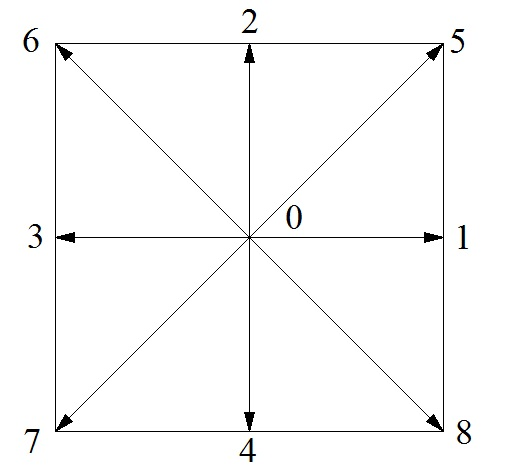
\includegraphics[]{figs/d2q9}
  \caption{D2Q9 lattice}
  \label{fig:d2q9}
\end{figure}

The discretized version of the Boltzmann equation, or the lattice Boltzmann equation (LBE), is given as: $f_i(\pos + \pvel_i, t + \Delta t) = f_i(\pos, t) + \cop_i(f)$, where, for D2Q9, $i = 0, 1, ..., 8$.

The macroscopic variables of interest can be calculated from the particle distribution functions, $f(\pos, \pvel, t)$, by integrating moments of $f$ over velocity space.
Due to the discrete nature of velocity in LBM, the integrals simply become summations.
The mass density is given by the sum of the particle distributions and the momentum density is given by the first moment of the particle distributions over the velocity space:

\begin{align}
\label{eq:rho} \rho(\pos, t) =& \sum_{i} f_i(\pos, t), \\
\label{eq:mom} \mmom(\pos, t) = \rho(\pos, t) \mvel(\pos, t) =& \sum_{i} \pvel_i(\pos, t) f_i(\pos, t)
\end{align}

The fluid pressure is related to macroscopic density through an equation of state:

\begin{equation}
\label{eq:pres} p(\pos, t) = \rho(\pos, t) c_s^2,
\end{equation}

\noindent where $c_s$ is the lattice speed of sound ($c_s = \frac{1}{\sqrt{3}}$, for D2Q9).

\subsection{Boundary Conditions}

No slip, or zero velocity, which is commonly imposed at walls in a domain, is accomplished by simulating the particle distributions as "bouncing back" at the walls in the opposite direction from which they stream.
For example, for a particle distribution streaming in the direction of a south wall, $f_2 = f_4$, $f_5 = f_7$, and $f_6 = f_8$.
For velocity or pressure boundary conditions, the method proposed by \citet{zou1997pressure} can be used.
The particle distributions that are missing after the streaming step are solved for by assuming a bounceback of the non-equilibrium distribution in the direction normal to the boundary; e.g., for a south inlet or outlet, $f_2 - f_2^{eq} = f_4 - f_4^{eq}$.

\subsection{Applied Forces}

Incorporating external forces, such as gravity, pressure gradients, etc., is done by adding a source of particle distributions in the direction of the force.
The increase in particle distributions leads to the desired macroscopic result--an increase in momentum.
The LBE with external forces is:

\begin{equation}
f_i(\pos + \pvel_i, t + \Delta t) = f_i(\pos, t) + \Omega_i(f) + \frac{w_i \Delta t}{c_s^2} \mathbf{F} \cdot \pvel_i
\end{equation}

\noindent where $\mathbf{F}$ is the body force vector.

\subsection{Collision Operator} %MG: if time allows, checkout differential lattice Bolzmann equation, the interpolation-supplemented lattice Boltzmann method, and the Taylor series expansion- and least square-based lattice Boltzmann method; Niu et. al. 2004

The collision operator, in the case of the continuous BE, attempts to describe the change in particle momentums and trajectories due to pairwise particle collisions (based on their respective momentums and trajectories just prior to collision) \cite{Cer90}.
In LBM, the collision operator causes particle distributions to relax toward a local equilibrium. This equilibrium is determined by the macroscopic physical behavior of interest.
In the case of incompressible flow, the equilibrium particle distribution, $f_i^{eq}$, is given by:

\begin{equation}
f_i^{eq} = w_i \rho \left[1 + \frac{\pvel_i \cdot \mvel}{c_s^2} + \frac{(\pvel_i \cdot \mvel)^2}{2c_s^2} - \frac{\mvel^2}{2c_s^2} \right]
\end{equation}

\noindent where $w_i$ is the weight in the $i^{th}$ direction.

\begin{equation*}
w_i = \begin{cases}
    \frac{4}{9}, & i = 0 \\
    \frac{1}{9}, & i = 1, 2, 3, 4 \\
    \frac{1}{36}, & i = 5, 6, 7, 8
\end{cases}
\end{equation*}

Due to its simplicity and computational efficiency, the most common collision operator is the Bhatnagar--Gross--Krook (BGK) operator.
BGK consists of a single relaxation time and is a linear relaxation of particle distributions toward equilibrium.
The BGK is expressed as:

\begin{equation}
\Omega_i = -\frac{1}{\tau} (f_i(\pos, t) - f_i^{eq}),
\end{equation}

\noindent where $\tau$ is the relaxation time \cite{Bha54}.
The relaxation time can be related to macroscopic constitutive properties through Chapman-Enskog multiscale analysis.
For incompressible Newtonian flow, the relaxation time is related to the kinematic viscosity by $\nu = c_s^2(\tau - \frac{1}{2})$.

An alternative to the BGK collision operator is the multiple-relaxation-time (MRT) collision operator.
%In the BGK collision scheme, high values of viscosity--such as those found in some cement slurry mixes--can lead to numerical instabilities \cite{svec2011flow,lallemand2000theory}.
Because the apparent viscosity can take on very large values without leading to numerical instabilities, the MRT collision operator has become popular for simulating non-Newtonian flows \cite{chen2014simulations,fallah2012multiple,tang2011bingham,vikhansky2008lattice,chai2011multiple}. %MG: is this necessary? wasn't this already covered
The MRT collision operator is given by:

\begin{equation} \label{eq:mrt-col-op}
	\cop = - {\transM}^{-1} \relaxM \transM (\mathbf{f} - \mathbf{f}^{eq}),
\end{equation}

where $\transM$ is a transformation matrix that maps the particle distribution vector, $\mathbf{f}$, and equilibrium distribution vector, $\mathbf{f}^{eq}$, from the particle distribution space into moment space, they will be denoted by $\mathbf{m}$ and $\mathbf{m}^{eq}$, respectively.
The relationships between $\mathbf{m}$, $\transM$ and $\mathbf{f}$ can be written as follows:

\begin{equation}
\mathbf{m} = \begin{bmatrix}
\rho \\ e \\ \epsilon \\ j_x \\ q_x \\ j_y \\ q_y \\ p_{xx} \\ p_{xy}
\end{bmatrix} = \begin{bmatrix}
1 & 1 & 1 & 1 & 1 & 1 & 1 & 1 & 1 \\
1 & 1 & 1 & 1 & 1 & 1 & 1 & 1 & 1 \\
1 & 1 & 1 & 1 & 1 & 1 & 1 & 1 & 1 \\
1 & 1 & 1 & 1 & 1 & 1 & 1 & 1 & 1 \\
1 & 1 & 1 & 1 & 1 & 1 & 1 & 1 & 1 \\
1 & 1 & 1 & 1 & 1 & 1 & 1 & 1 & 1 \\
1 & 1 & 1 & 1 & 1 & 1 & 1 & 1 & 1 \\
1 & 1 & 1 & 1 & 1 & 1 & 1 & 1 & 1 \\
1 & 1 & 1 & 1 & 1 & 1 & 1 & 1 & 1
\end{bmatrix}
\end{equation}

\subsubsection{Entropic Collisions and Entropy Balance}

\section{Numerical Study}

\subsection{Poiseuille Flow} 

\subsection{Lid-driven Flow}

\section{Conclusion}

\section*{Acknowledgements}

\bibliographystyle{abbrvnat}
\bibliography{master}
	
\end{document}
